\documentclass{article}
\usepackage{clrscode3e}
\usepackage[margin=1in]{geometry}
\usepackage{amsfonts,amsmath}
\usepackage{graphicx}
\usepackage{fancyvrb}
\usepackage{hyperref}


\newcommand{\R}{\mathbb{R}}
\newcommand{\N}{\mathbb{N}}

\title{Some \LaTeX{}  examples}
\author{Geoffrey Matthews}

\begin{document}
\maketitle

\section{Mechanics}
This file contains some examples to get you started using \LaTeX{} to
typeset mathematics.  It is the premiere software for technical
publications.  Good places to get started:
\begin{itemize}
\item \url{http://www.latex-tutorial.com/}
\item \url{http://www.stdout.org/~winston/latex/latexsheet.pdf}
\end{itemize}

To compile a \LaTeX{} file, {\tt myfile.tex} to {\tt myfile.pdf}, 
simply enter the
following command:
\begin{Verbatim}[frame=single]
pdflatex myfile.tex
\end{Verbatim}
or use a GUI such as TexWorks or TexStudio.

You can also get your \LaTeX\ processed online, for example, at \url{https://www.overleaf.com/}

\section{Some example text}
Here is some inline math:  $\sum_{i=1}^{n} i^2$ and
here is the same thing with display math:
\[
\sum_{i=1}^{n} i^2
\]
Here is a set of equations lined up nicely:
\begin{align*}
(a+b)^2 &= (a+b)(a+b) \\
        &= a(a+b) + b(a+b) \\
        &= a^2 + ab + ba + b^2 &\mbox{Here's a comment on a line}\\
        &= a^2 + 2ab + b^2     &\mbox{Simple proof!}
\end{align*}

You can talk about the real numbers, $\R$, the integers $\mathbb{Z}$, the
rational numbers $\mathbb{Q}$, and the natural numbers,
$\N$, using nice fonts.  Notice how I made new commands for some of these in
the preamble, to simplify typing.
Here is an enumerated list:
\begin{enumerate}

\item $\mathcal{P}(\{1,2,3\}) \subseteq \mathcal{P}(\{1,2,3,4\})$

\item
$
\bigcup_{i\in\N}i^2 = \{0,1,4,9,\ldots\} = \{n^2 \mid n \in \mathbb{N}\}
$

\item
\[
\bigcap_{i\in\N}i^2 \not= \{0,1,4,9,\ldots\}
\]

\end{enumerate}

\section{Figures}
You can also include and scale figures:

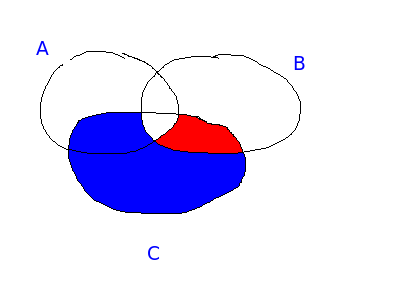
\includegraphics[scale=0.5]{sets.png}

\section{Algorithms}


  If you're using the CLRS book in an algorithms class, you can
download the {\tt clrscode3d.sty} file and use it like this:
\begin{Verbatim}[frame=single]
  \usepackage{clrscode3d.sty}
  \end{Verbatim}
\begin{minipage}{0.575\textwidth}
and then you can enter the code on the left to get the algorithm on the right:
\begin{Verbatim}[frame=single]
\begin{codebox}
\Procname{$\proc{Insertion-Sort}(A)$}
\li \For $j \gets 2$ \To $\attrib{A}{length}$
\li
\Do
$\id{key} \gets A[j]$
\li
\Comment Insert $A[j]$ into the sorted sequence
$A[1 \twodots j-1]$.
\li
$i \gets j-1$
\li
\While $i > 0$ and $A[i] > \id{key}$
\li
\Do
$A[i+1] \gets A[i]$
\li
$i \gets i-1$
\End
\li
$A[i+1] \gets \id{key}$
\End
\end{codebox}
\end{Verbatim}
\end{minipage}
\begin{minipage}{0.475\textwidth}
\begin{codebox}
\Procname{$\proc{Insertion-Sort}(A)$}
\li \For $j \gets 2$ \To $\attrib{A}{length}$
\li
\Do
$\id{key} \gets A[j]$
\li
\Comment Insert $A[j]$ into the sorted sequence
$A[1 \twodots j-1]$.
\li
$i \gets j-1$
\li
\While $i > 0$ and $A[i] > \id{key}$
\li
\Do
$A[i+1] \gets A[i]$
\li
$i \gets i-1$
\End
\li
$A[i+1] \gets \id{key}$
\End
\end{codebox}
\end{minipage}

\end{document}
